% Titlepage
\begin{titlepage}
	\begin{center}
		\Huge{\textbf{That's it}}\\
		\LARGE{Kleiner Leitfaden für Erstsemester}
		\vfil
		
\includegraphics[width=0.6\textwidth]{\imgdir/prof.png}
		\vfil
		\LARGE{\semester}
	\end{center}
\end{titlepage}

% Rückseite der Titlepage; pagestyle{empty}: keine Kopf- und Fußzeile
\pagestyle{empty}
\begin{figure}
	\begin{center}
		
\includegraphics[width=\textwidth]{\imgdir/Phi.pdf}
	\end{center}
\end{figure}
\pagebreak

% Einbindung des Vorworts; \chapdir verweist auf den im header definierten kapitel-Ordner.
\section{Vorwort}

\hspace{0.5cm} Hallo!

Raus aus der Schule und rein ins Vergnügen. Nach 12 Jahren
langweiligen Deutschunterrichts und unzähligen Sozialkundestunden habt ihr es nun geschafft, an die Schwelle der unendlich hohen Treppe der Wissenschaft vorzuschreiten.

Ein neuer Lebensabschnitt der Arbeit, Verzweiflung, Frustration, aber auch der Freude liegt nun direkt vor euch und die Furien an euren Füßen warten schon darauf, euch in ihren Bann des ewigen Wahnsinns zu ziehen.

Noch liegt all dies zwar in der Zukunft, aber wie immer schreitet die Zeit voran wie ein großer gekoppelter harmonischer Oszillator ohne Randbedingungen.
Und wenn ihr heute noch lachen könnt über die üblichen
bösen Kommentare zu eurem Studium, wie z.B. von der amüsierten
Mutter: \glqq Ein bisschen Studieren und abends Party machen \ldots \grqq , so wird sich doch diese Meinung in der nächsten Zeit wandeln. Denn um es zusammenzufassen, habt ihr nun ASS und das steht nicht für ein Erkältungsmittel sondern für Arbeit, Stress und nochmal Stress. Also genießt nochmal das letzte freie Bier eures Lebens und auf in die Schlacht\ldots

\begin{figure}[b!]
\begin{center}
  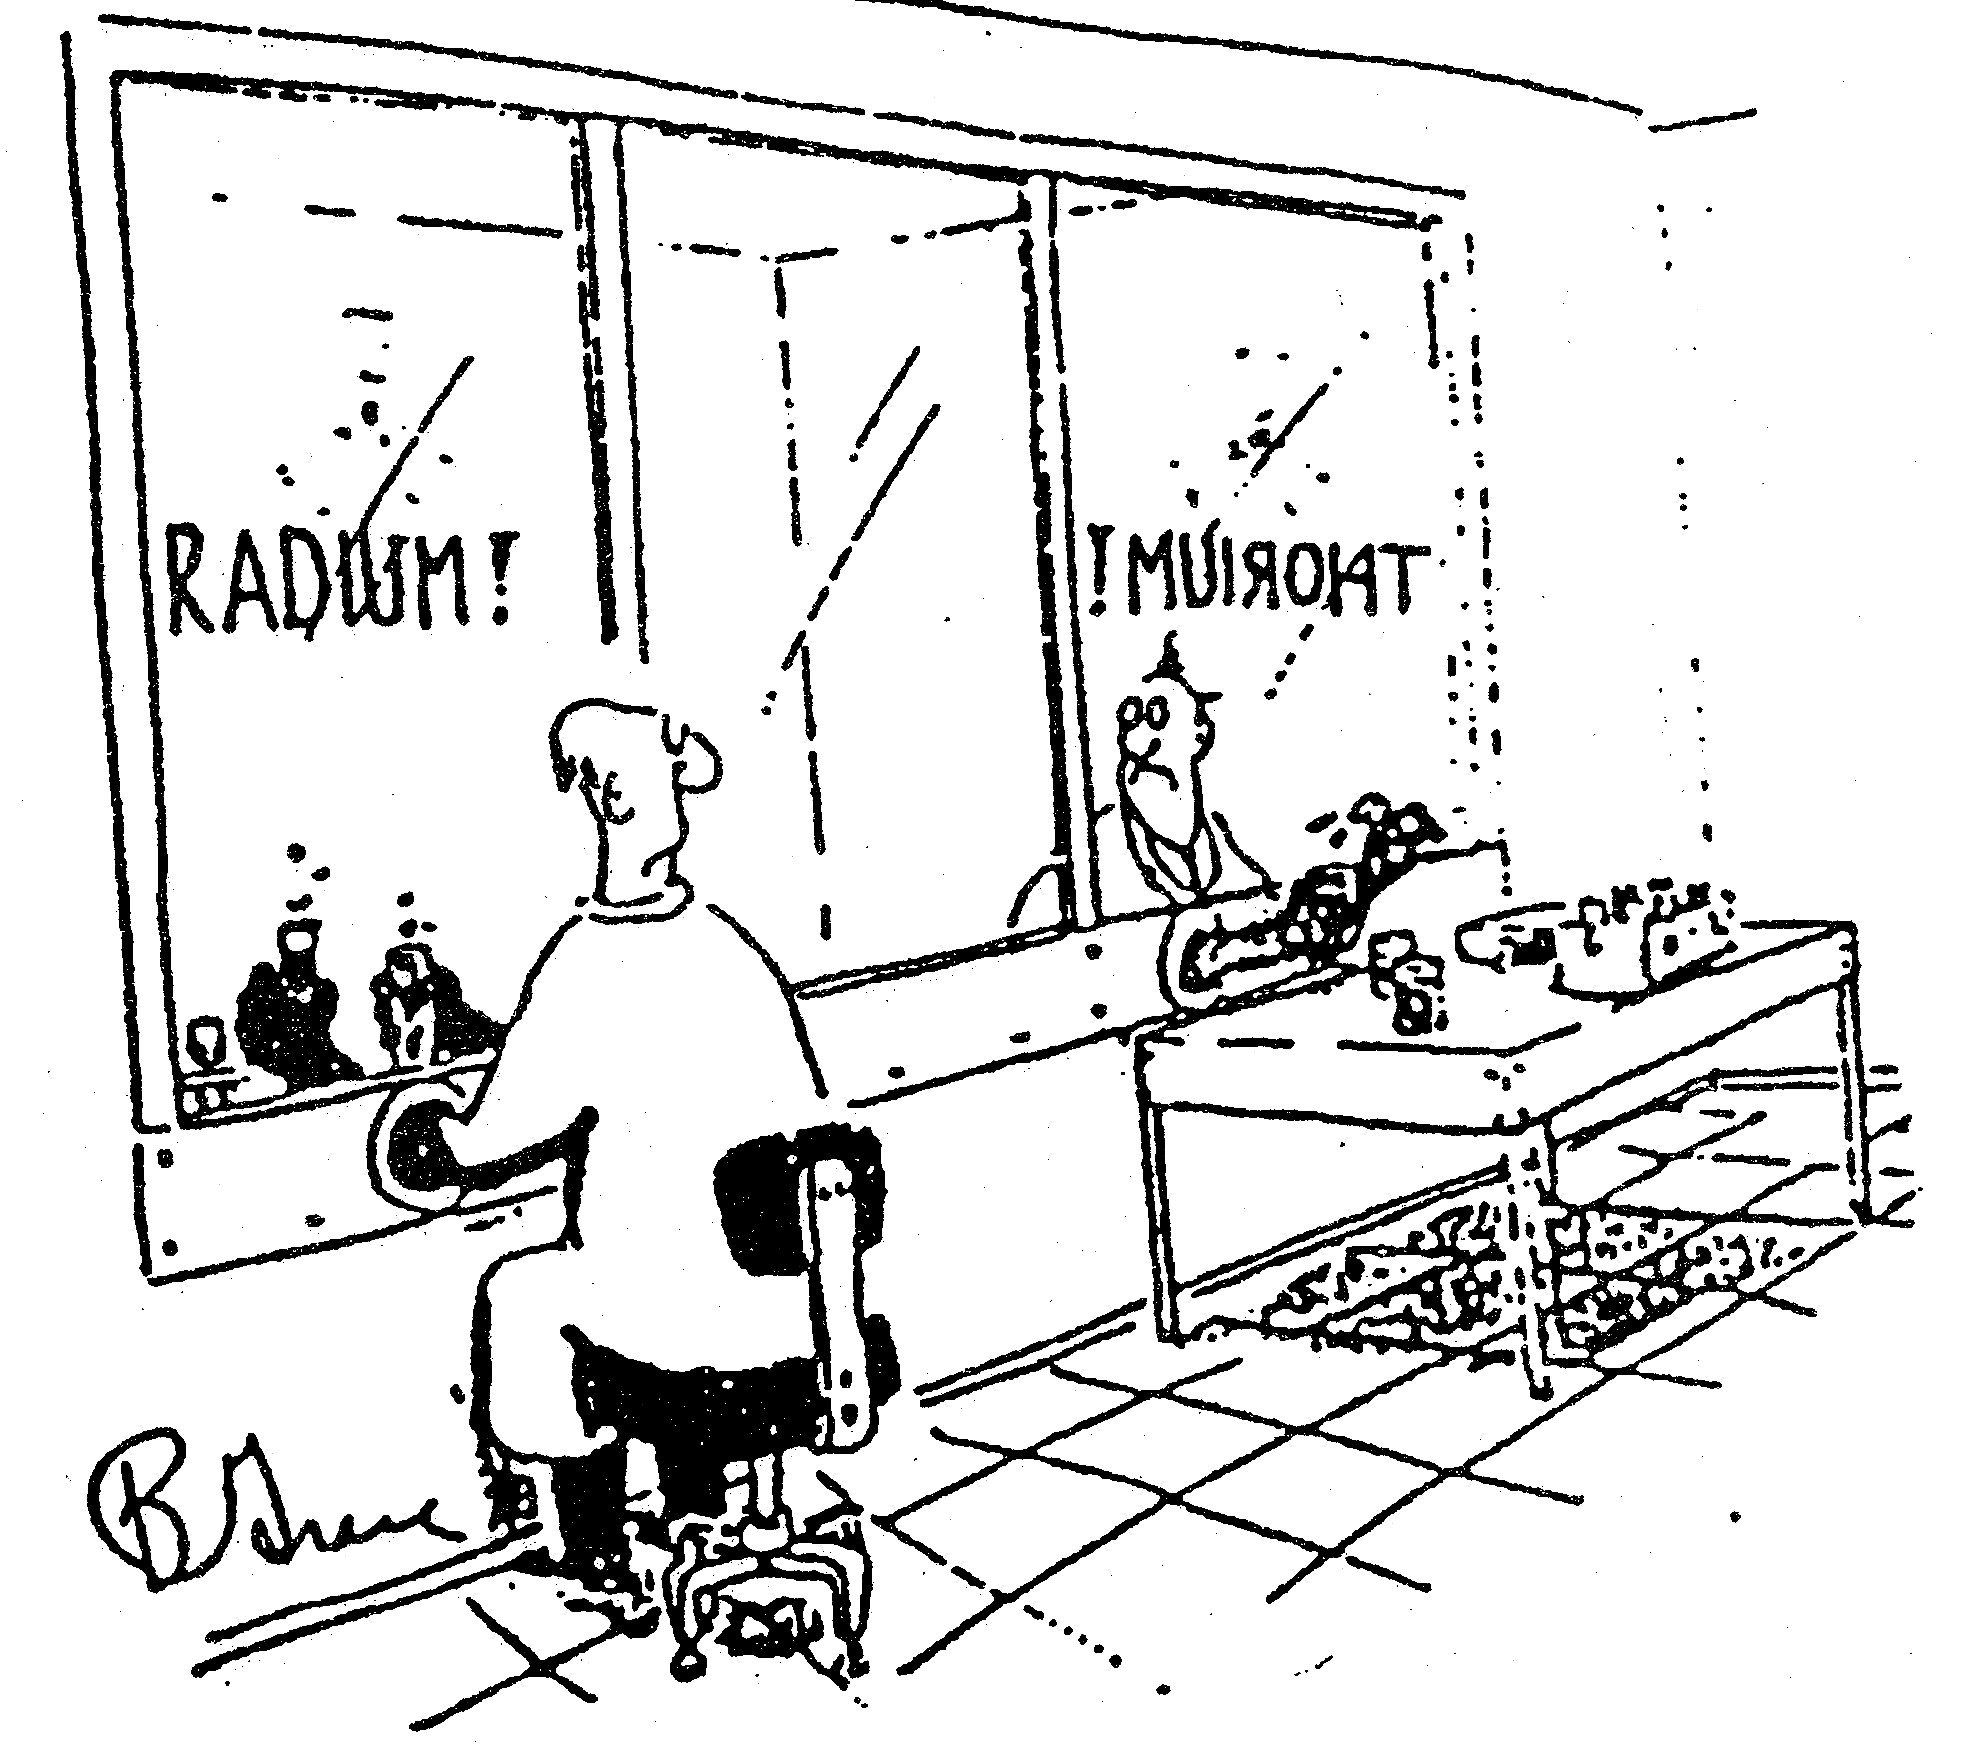
\includegraphics[width=.45\textwidth]{bilder/radium-thorium.jpg}
\end{center}
\end{figure}

So, das war nun die \glqq Das-Leben-ist-ungerecht-und-alles-ist-so-schwer-Seite\grqq . Aber zum Glück gibt es da ja noch die \glqq Physik-ist-toll-Seite\grqq . Und diese überwiegt definitiv die andere, da ihr euch das beste, interessanteste und umfassenste Studienfach ausgesucht habt, das es gibt.
Denn wenige Biologen werden euch erklären können, was ein Photon ist, noch weniger Chemiker, wie Quantenmechanik funktioniert, fast kein BWLer, wie man rechnet, und kein Jurist, wie man Partys feiert.

Also schätzt euch glücklich.
Und auf den Spruch: \glqq Physiker haben doch keine Freunde\grqq könnt ihr bald getrost antworten: 
\glqq Doch! Und zwar verdammt viele andere Physiker.\grqq

In diesem Sinne: \textbf{Herzlich Willkommen} in der Physik!
